\section{Introducción}


\begin{frame}
\frametitle{Motivación}

\begin{block}{Objetivo a desarrollar}
Método de reconstrucción 3D o mapeo denso en tiempo real sobre sistemas de localización y mapeo simultáneo (SLAM) basado en visión estéreo.
\end{block}

\end{frame}


\begin{frame}
\frametitle{Reconstrucción 3D}

\pnote{Reconstrucción 3D: Proceso mediante el cual se captura y representa la forma y apariencia de entornos u objetos presentes en la realidad. Diseño asistido por computadora, imágenes médicas, realidad virtual y aumentada, robótica movil, entre otros.}

\begin{figure}[!htb]
	\centering
	\subfloat[]{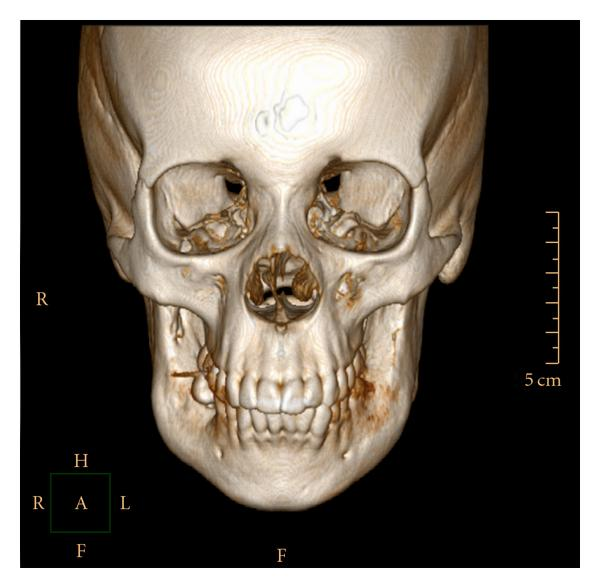
\includegraphics[width=0.30\columnwidth]{./introduction/3d-skull.jpg}}%
	\hfill
	\subfloat[]{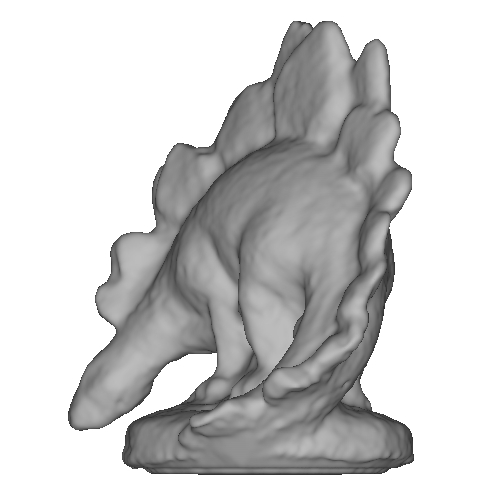
\includegraphics[width=0.30\columnwidth]{./introduction/3d-dinosaur.jpg}}%
	\hfill
	\centering
	\subfloat[]{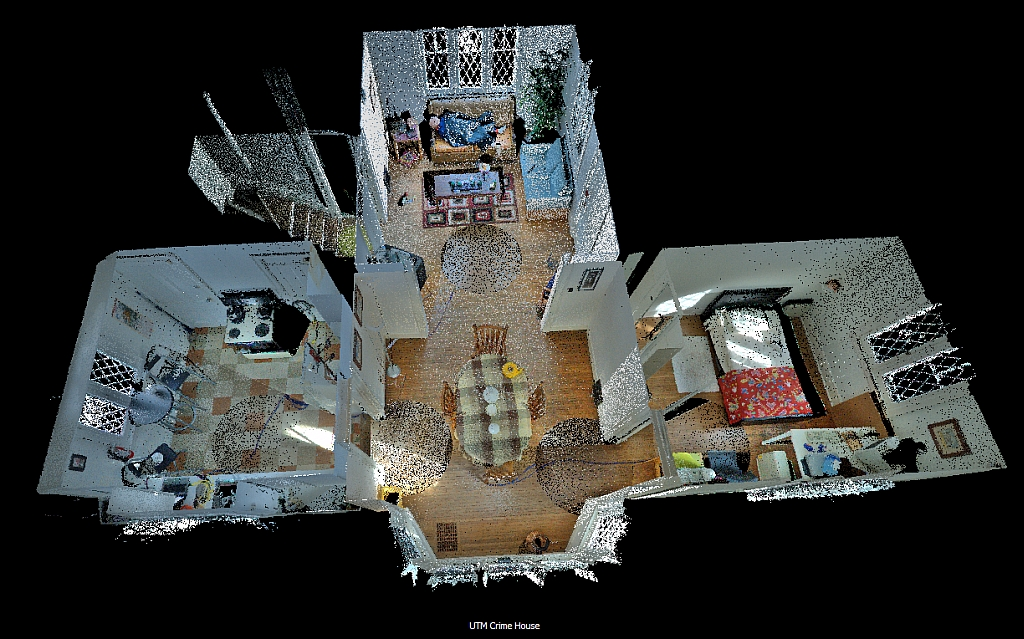
\includegraphics[width=0.40\columnwidth]{./introduction/3d-indoor.jpg}}%
	\hfill
	\\
	\centering
	\subfloat[]{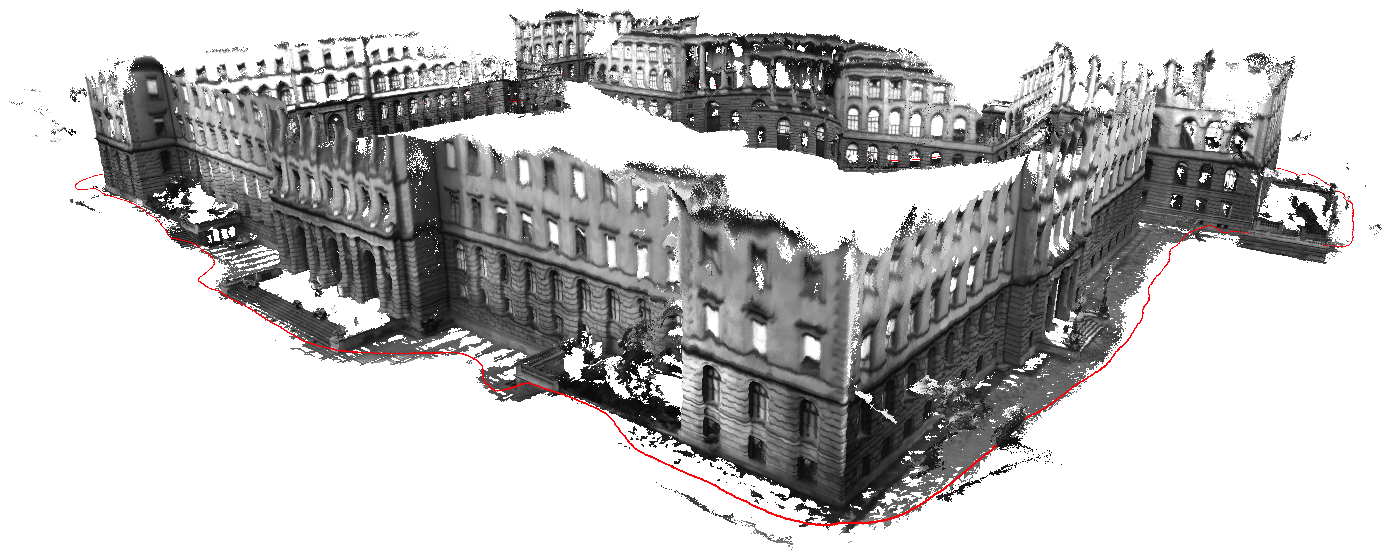
\includegraphics[width=0.70\columnwidth]{./introduction/3d-building.png}}%
	\hfill
\end{figure}

\end{frame}


\begin{frame}
\frametitle{SLAM - Simultaneous Localisation and Mapping}

\pnote{A partir de la detección y seguimiento de marcas naturales del ambiente (landmarks), los sistemas de SLAM pueden estimar tanto la posición del robot como la ubicación de estas marcas en el entorno. El mapa es construído incrementalmente con las posiciones estimadas de dichas marcas, las cuales son ajustadas a lo largo de la trayectoria a medida que son observadas.}

\begin{itemize}
\item Construir incrementalmente un mapa del entorno.
\item Determinar su posición y orientación en el mismo.
\end{itemize}

\begin{figure}[!htb]
	\centering
	\subfloat[]{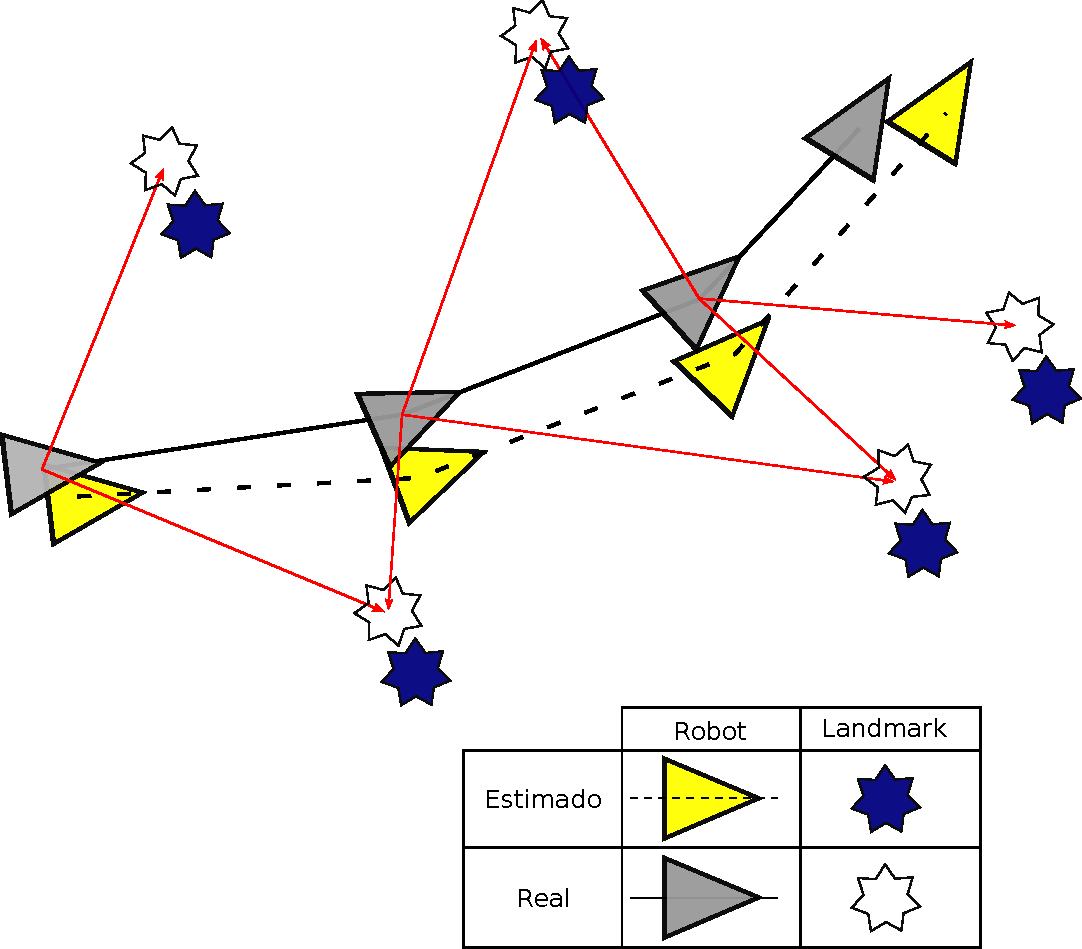
\includegraphics[width=0.50\columnwidth]{./introduction/slam-landmarks.pdf}}%
	\hfill
\end{figure}

\end{frame}


\begin{frame}
\frametitle{SLAM Visual - Cámaras}

\pnote{Cámaras: rica información de la escena. Ventajas: bajo costo, menor consumo energético en comparación con otros sensores, como lásers, portabilidad y alta disponibilidad en dispositivos móviles. Son sensores pasivos por lo que no interferen con otros sensores y pueden utilizarse en entornos interiores, donde el uso de GPS puede verse imposibilitado. Asímismo, son menos restrictivos que los encoders, los cuales se encuentran limitados a robots terrestres y resultan imprecisos en terrenos irregulares.}

\begin{itemize}
\item Bajo costo.
\item Bajo consumo energético.
\item Alta disponibilidad en dispositivos móviles.
\item Sensores pasivos.
\item Apto entornos interiores.
\item Apto terrenos irregulares.
\end{itemize}

\end{frame}


\begin{frame}
\frametitle{SLAM Visual - Cámaras estéreo}

\pnote{Cámaras estéreo: Existen dos enfoques predominantes en los sistemas de SLAM basados en cámaras, denominados monocular y estéreo. Los sistemas de SLAM visual estéreo proveen información sobre la profundidad de los píxeles mediante una única observación, lo cual requiere mayor número de cómputos en el caso monocular.}

\begin{figure}[!htb]
	\centering
	\subfloat[]{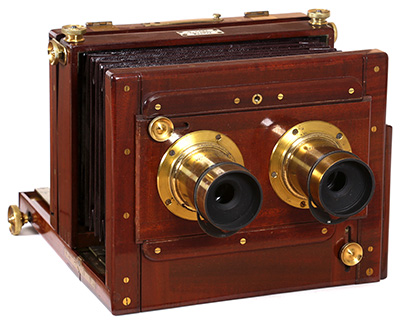
\includegraphics[width=0.45\columnwidth]{./introduction/camera-stereo-old.jpg}}%
	\hfill
	\centering
	\subfloat[]{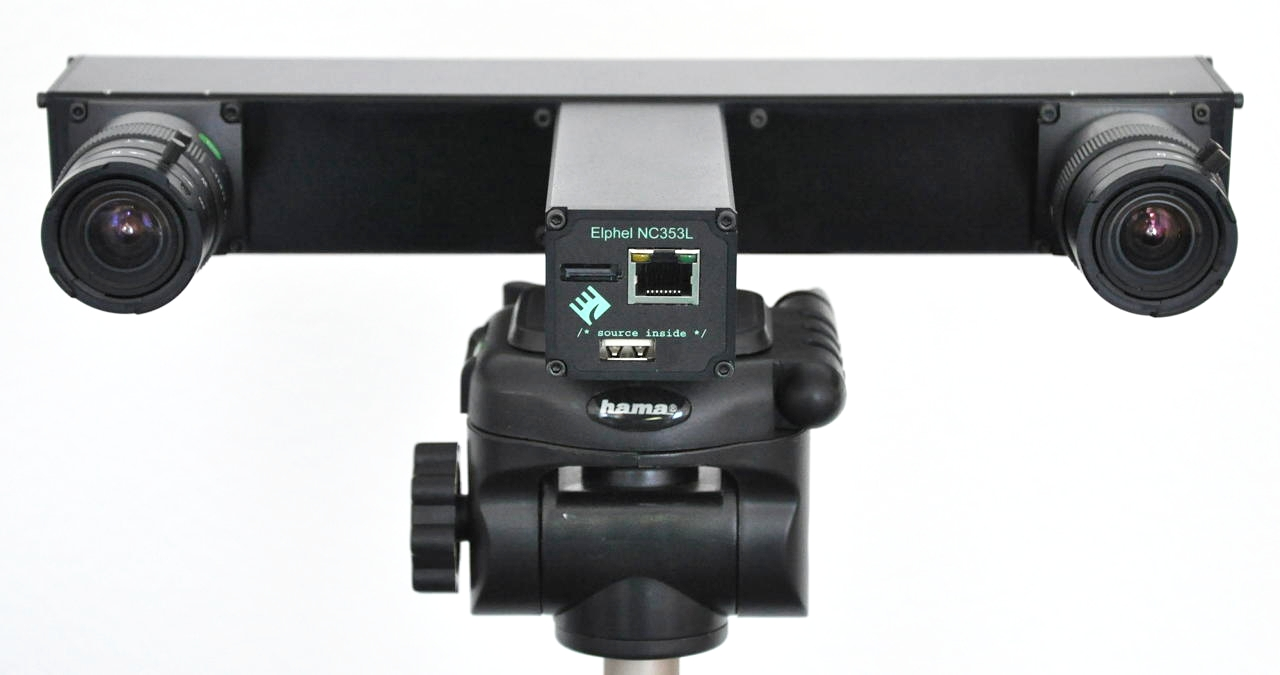
\includegraphics[width=0.45\columnwidth]{./introduction/camera-stereo-new.jpg}}%
	\hfill
\end{figure}

\end{frame}